\documentclass[12pt]{article}

% UTF-8 encoding and fonts
\usepackage[utf8]{inputenc}
\usepackage[T1]{fontenc}
\usepackage{lmodern}

% Page setup
\usepackage[margin=1in]{geometry}
\usepackage{setspace}
\onehalfspacing

% Typography
\usepackage{microtype}

% Math and symbols
\usepackage{amsmath,amssymb}

% Graphics
\usepackage{graphicx}
\usepackage{float}
\usepackage{subcaption}

% Tables
\usepackage{booktabs}
\usepackage{array}
\usepackage{multirow}
\usepackage{threeparttable}
\usepackage{longtable}
\usepackage{pdflscape}
\usepackage{siunitx}
\sisetup{detect-all=true, group-separator={,}, group-minimum-digits=4}

% Bibliography
\usepackage{natbib}
\bibliographystyle{aer}

% Hyperlinks
\usepackage{hyperref}
\hypersetup{
    colorlinks=true,
    linkcolor=blue,
    citecolor=blue,
    urlcolor=blue
}
\usepackage[nameinlink,noabbrev]{cleveref}

% Timing data
\IfFileExists{timing_data.tex}{\input{timing_data.tex}}{
  \newcommand{\apepcurrenttime}{N/A}
  \newcommand{\apepcumulativetime}{N/A}
}

% Captions
\usepackage{caption}
\captionsetup{font=small,labelfont=bf}

% Section formatting
\usepackage{titlesec}
\titleformat{\section}{\large\bfseries}{\thesection.}{0.5em}{}
\titleformat{\subsection}{\normalsize\bfseries}{\thesubsection}{0.5em}{}

% Custom commands
\newcommand{\E}{\mathbb{E}}
\newcommand{\Var}{\text{Var}}
\newcommand{\Cov}{\text{Cov}}
\newcommand{\ind}{\mathbb{I}}
\newcommand{\sym}[1]{\ifmmode^{#1}\else\(^{#1}\)\fi}

\title{Vacancy Taxes and Housing Markets: Evidence from France's 2023 TLV Expansion}
\author{APEP Autonomous Research\thanks{Autonomous Policy Evaluation Project. Correspondence: scl@econ.uzh.ch{} (cumulative: \apepcumulativetime{}).} \and @olafdrw}
\date{\today}

\begin{document}

\maketitle

\begin{abstract}
\noindent
Can vacancy taxes cool overheated housing markets in tourism-dependent areas? I exploit France's 2023 expansion of the Taxe sur les Logements Vacants (TLV), which newly designated 2,590 communes for vacancy taxation effective January 2024, to estimate effects on property prices and transaction volumes. Using 4.1 million property transactions from 2020--2025, I find that the expansion reduced transaction volume by 6.0\% but had no robust effect on commune-level prices. Transaction-level estimates suggest a 2.8--3.7\% price increase, but this is consistent with compositional selection as cheaper properties exit the market. The strongest effect appears in 2023---before the tax took effect---suggesting anticipation or signaling. Tourism communes drive the modest price response; non-tourism communes show null effects. The results suggest vacancy taxes primarily reduce market liquidity rather than prices.
\end{abstract}

\vspace{1em}
\noindent\textbf{JEL Codes:} H71, R21, R31, R38 \\
\noindent\textbf{Keywords:} vacancy tax, housing policy, property markets, difference-in-differences, France, tourism housing

\newpage

\section{Introduction}

In the resort towns of the French Riviera, one in five homes sits empty for most of the year. Meanwhile, the Fondation Abb\'e Pierre estimates that 4.2 million people across France are poorly housed or homeless \citep{fondation2023}. Nationally, 3.1 million dwellings --- 8.3\% of the housing stock --- stand vacant \citep{cour2023}. This collision of scarcity and surplus has driven a series of increasingly aggressive fiscal interventions, culminating in the massive expansion of France's vacancy tax in August 2023.

The Taxe sur les Logements Vacants (TLV) was introduced in 1999, initially covering about 1,100 communes in the largest urban agglomerations. D\'ecret n\textsuperscript{o} 2023-822 \citep{dgfip2023}, published on August 25, 2023, dramatically expanded the TLV's geographic scope by adding approximately 2,590 communes --- predominantly coastal, mountain, and tourism-dependent areas classified as ``zones tendues'' (tight housing markets). Simultaneously, the tax rates were increased from 12.5\% to 17\% of cadastral rental value in the first year and from 25\% to 34\% thereafter. This expansion became effective on January 1, 2024, providing a clean treatment date for empirical analysis.

This paper estimates the causal effect of the TLV expansion on housing prices and transaction volumes using a difference-in-differences design. The treatment group consists of the 2,590 communes newly designated under D\'ecret 2023-822. The control group consists of the 31,147 communes that were never subject to the TLV (of which 29,447 have at least one DVF transaction in the sample period). I exclude the approximately 1,100 communes that had been in the TLV regime prior to 2023, as they face a different treatment history. The primary outcome data come from the Demandes de Valeurs Fonci\`eres (DVF), France's universe of notarized property transactions, covering 4.1 million residential sales from 2020 to 2025.

The results present a nuanced picture. The most robust finding is a significant reduction in transaction volume: the TLV expansion reduced the log number of residential sales in treated communes by 0.060 (approximately 5.8\%) in the baseline specification, significant at the 1\% level. With the more stringent d\'epartement $\times$ year fixed effects, the estimate attenuates to 0.028 but remains significant at the 5\% level. This finding is consistent with the theoretical prediction that higher holding costs reduce market turnover by discouraging discretionary sales.

The evidence on prices is more equivocal. At the commune-year level, the preferred specification yields a point estimate of 1.2\% with a standard error of 0.8\% --- economically small and statistically indistinguishable from zero. When I saturate the model with d\'epartement $\times$ year fixed effects, the estimate falls further to 0.8\% (p = 0.31). At the transaction level, where individual property sales are the unit of observation, the estimates are larger and statistically significant: 3.7\% with commune and year fixed effects, 2.8\% with d\'epartement $\times$ year fixed effects. The divergence between commune-level and transaction-level estimates is itself informative: when volume falls but transaction-level prices rise, the natural interpretation is compositional selection --- the properties that stop trading are disproportionately lower-valued.

An event-study specification reveals that the strongest effect appears in 2023, the year the expansion was \textit{announced} but before it took effect. The 2023 coefficient of 2.9\% is highly significant, while the 2024 and 2025 coefficients (1.4\% and 1.8\%) are individually insignificant. This pattern is consistent with an anticipation or signaling mechanism: the designation of a commune as a ``zone tendue'' may itself be interpreted by market participants as a signal of housing scarcity, influencing expectations and prices independently of the tax's direct fiscal impact.

Heterogeneity analysis reveals that the expansion's effects are concentrated in tourism-dependent communes (``zones touristiques et tendues''), which account for 87\% of newly designated communes. Tourism communes show a marginally significant price increase of 1.7\% (p = 0.054), while non-tourism communes exhibit a precisely estimated null effect ($-$1.1\%, p = 0.23). This pattern suggests that the TLV may interact with the amenity value of tourism locations --- the designation itself may reinforce market expectations about the desirability and scarcity of housing in these areas.

This paper contributes to several literatures. First, it extends the growing literature on housing taxation, which has primarily focused on transaction taxes \citep{best2020, dachis2012, kopczuk2006} and property taxes \citep{saarimaa2012, eerola2021}. Vacancy taxes are a distinct instrument with different behavioral margins: rather than taxing transactions, they tax \textit{inaction} --- the decision not to rent or sell. The theoretical predictions differ accordingly, and empirical evidence is scarce. \citet{gravel2019} provide the only prior evaluation of the French TLV, finding modest effects in the original urban zones, but the 2023 expansion to tourism communes represents a fundamentally different economic context.

Second, the paper contributes to the literature on housing supply regulation and its price effects \citep{saiz2010, hilber2016, hsieh2019}. While most of this literature examines supply restrictions that raise prices, vacancy taxes are designed to \textit{increase} effective supply by mobilizing empty units. The finding that prices do not fall --- and may modestly rise --- suggests that the supply-side channel is weak, at least in the short run. This is consistent with the hypothesis that many ``vacant'' properties in tourism communes are second homes whose owners absorb the tax rather than rent or sell.

Third, I contribute to the literature on anticipation and announcement effects in housing markets \citep{mian2009, adelino2015}. The finding that the TLV's market impact materializes upon announcement rather than implementation suggests that housing market participants respond to information about future policy regimes --- the ``zone tendue'' designation itself carries informational content about local market conditions.

Finally, the paper contributes methodologically. With 2,590 treated communes and 29,447 controls observed over six years, the design satisfies the demanding requirements for credible DiD inference outlined by \citet{bertrand2004}. I complement the standard TWFE estimator with randomization inference \citep{fisher1935}, propensity score matching, and extensive robustness checks including placebo tests, donut regressions, and d\'epartement $\times$ year fixed effects.

The paper also speaks to a broader policy debate about how governments should address housing affordability in tourism-dependent communities. From the Basque coast to the Alps, from Brittany to Provence, the tension between permanent residents' need for affordable housing and the economic benefits of tourism and second-home ownership is one of the defining challenges of French territorial policy. The TLV expansion represents one approach to this tension --- using fiscal instruments to discourage vacancy and increase effective housing supply. Understanding whether this approach works, and through what channels, is essential for evidence-based housing policy in France and internationally.

\section{Institutional Background}

\subsection{The French Vacancy Tax: Origins and Evolution}

France's Taxe sur les Logements Vacants was created by the Loi de Lutte contre les Exclusions of July 29, 1998 (Article 232 of the Code G\'en\'eral des Imp\^ots). The tax targets residential dwellings that have been vacant for at least one year, defined as properties that are neither occupied as a primary residence, used as a secondary residence, nor rented. The TLV applies specifically to communes located in ``zones d'urbanisation continue de plus de 200,000 habitants'' --- continuously urbanized areas with populations exceeding 200,000 where there is a ``marked imbalance between housing supply and demand.''

The initial 1999 implementation covered communes in eight major agglomerations (Paris, Lyon, Marseille, Lille, Bordeaux, Toulouse, Montpellier, and Nice), totaling approximately 811 communes. The tax was levied on the cadastral rental value of the property: 10\% in the first year of vacancy, 12.5\% in the second year, and 15\% from the third year onward. Revenue flowed to the Agence Nationale de l'Habitat (ANAH), not to local governments, eliminating any fiscal incentive for communes to strategically seek designation.

In 2013, D\'ecret n\textsuperscript{o} 2013-392 expanded the TLV to 28 ``zones tendues'' covering approximately 1,151 communes. The expansion targeted agglomerations with populations exceeding 50,000 where construction was insufficient to meet housing demand. Tax rates were simultaneously increased to 12.5\% (first year) and 25\% (subsequent years).

\subsection{The 2023 Expansion}

D\'ecret n\textsuperscript{o} 2023-822, published in the Journal Officiel on August 25, 2023, represented the most significant expansion of the TLV in its history. The decree added approximately 2,590 communes to the TLV regime effective January 1, 2024, and raised the tax rates to 17\% (first year) and 34\% (subsequent years). The expansion was motivated by the recognition that housing market pressures extended well beyond traditional urban agglomerations into tourism-dependent areas, particularly coastal and mountain communes.

The newly designated communes fall into two categories within the zonage classification:
\begin{itemize}
    \item \textbf{Zones tendues} (330 communes): Areas identified as tight housing markets based on supply-demand imbalance criteria, but not primarily defined by tourism activity.
    \item \textbf{Zones touristiques et tendues} (2,260 communes): Areas where housing market tension is compounded by significant seasonal tourism demand, typically characterized by high rates of secondary home ownership.
\end{itemize}

The dominance of ``zones touristiques et tendues'' (87\% of newly designated communes) reflects the policy's primary target: communities where second-home ownership and seasonal vacancy reduce the effective housing stock available to permanent residents. These communes trace a distinctive geography: the crowded beaches of the Mediterranean (Var, Alpes-Maritimes, H\'erault), the Atlantic coast from Charente-Maritime to Vend\'ee, and the ski slopes of the Alps (Haute-Savoie, Savoie) and Pyr\'en\'ees.

\subsection{Mechanisms and Expected Effects}

The TLV operates through several channels. The direct channel is fiscal: owners of vacant properties face an annual tax liability equal to 17--34\% of the property's cadastral rental value, creating an incentive to either rent the property, sell it, or occupy it. For a property with a cadastral value of \euro{5,000}, the annual TLV liability would range from \euro{850} to \euro{1,700} --- a non-trivial amount for lower-value properties but potentially inconsequential for high-value second homes in desirable tourism locations.

The expected effects on housing markets are theoretically ambiguous. On the supply side, the TLV should increase the effective supply of housing (through rental or sales), which would put downward pressure on prices. On the demand side, the ``zone tendue'' designation may act as a quality signal, confirming to potential buyers that the commune is a desirable location with genuine housing scarcity. This signaling channel would push prices upward. The net effect is an empirical question.

Transaction volumes could move in either direction. If owners respond to the TLV by selling vacant properties, volumes should increase. However, if the tax reduces the attractiveness of holding property as an investment or second home, potential buyers may be deterred, reducing volume. The composition of transactions may also shift: if the properties brought to market by the TLV are typically older, smaller, or lower-quality than the pre-existing transaction mix, observed average prices would change even without any change in the price of comparable properties.

A critical feature of the 2023 expansion is the August 25 announcement date for a January 1, 2024 effective date. This four-month window creates potential for anticipation effects. Rational property owners, upon learning of their commune's designation, may have accelerated or delayed sales, adjusted asking prices, or shifted rental decisions before the tax actually took effect.

\subsection{International Context}

Vacancy taxes are not unique to France. Vancouver introduced a 1\% Empty Homes Tax in 2017 (later raised to 3\%), and the Canadian federal government implemented a 1\% Underused Housing Tax on foreign-owned vacant properties in 2022. Melbourne introduced a similar levy in 2018. In all cases, the policy motivation is similar: to discourage holding property vacant in markets where housing affordability is a pressing concern. However, the French TLV is distinctive in several respects.

First, the French tax applies to all vacant properties regardless of the owner's nationality or residency status, targeting the \textit{vacancy decision} rather than the owner's characteristics. Second, the TLV rates (17--34\% of cadastral value) are substantially higher than most international comparisons when measured against imputed rental income. Third, the 2023 expansion specifically targeted tourism and secondary-home markets, a context that differs from the urban vacancy addressed by Vancouver and Melbourne.

The French system also interacts with other fiscal instruments for housing. Communes may independently vote to apply the Taxe d'Habitation sur les Logements Vacants (THLV), a separate vacancy surtax under Article 1407 bis of the Code G\'en\'eral des Imp\^ots. Additionally, properties classified as ``secondary residences'' rather than ``vacant'' are subject to the taxe d'habitation sur les r\'esidences secondaires, which communes in zones tendues can surcharge by up to 60\%. The boundary between ``vacant'' and ``secondary residence'' is often fuzzy in tourism areas, creating opportunities for reclassification that may attenuate the TLV's effectiveness.

\subsection{Political Economy of the 2023 Expansion}

The 2023 expansion was preceded by extensive political debate. Mayors of coastal and mountain communes had lobbied for years to be included in the TLV perimeter, arguing that seasonal vacancy was distorting local housing markets and displacing permanent residents. The expansion was announced as part of a broader housing policy package by the Ministry of Ecological Transition, which framed it as a response to the ``structurally tight'' housing markets identified in the Rapport Kasbarian-Bergé (2023) on housing market dysfunction.

The political economy is relevant for identification because it means that treatment assignment was partly driven by local political pressure rather than purely technocratic criteria. Communes with more politically active mayors or stronger housing advocacy may have been more likely to be designated. If these communes were also on different price trajectories, this could bias the estimates. The d\'epartement $\times$ year specification addresses this concern by absorbing regional-level political dynamics, but within-d\'epartement political variation remains a potential source of confounding.


\section{Conceptual Framework}

Consider a simple model of vacant property holding. A property owner in commune $c$ at time $t$ chooses among three options: rent the property (earning net rental income $r_{ct}$), sell the property (receiving price $P_{ct}$ minus transaction costs $\tau$), or hold it vacant (receiving an amenity or option value $v_{ct}$ minus the TLV liability $T_{ct}$). The owner holds the property vacant when:
\begin{equation}
    v_{ct} - T_{ct} > \max\{r_{ct}, P_{ct} - \tau\}
\end{equation}

The introduction of the TLV increases $T_{ct}$ from zero to $\theta \cdot RV_c$, where $\theta \in \{0.17, 0.34\}$ is the tax rate and $RV_c$ is the cadastral rental value. This reduces the net benefit of vacancy and should, at the margin, push some owners toward renting or selling. The equilibrium effect on prices depends on the elasticity of local housing supply and demand.

\textbf{Prediction 1:} Transaction volume should increase in newly taxed communes if the supply effect dominates (owners offloading vacant properties), or decrease if the demand effect dominates (reduced investment demand).

\textbf{Prediction 2:} Prices should decrease if the TLV primarily mobilizes vacant properties for sale or rent (supply expansion), or remain unchanged if owners absorb the tax.

\textbf{Prediction 3:} The signaling channel predicts that prices may increase if the ``zone tendue'' designation is interpreted as confirming housing market tightness.

\textbf{Prediction 4:} Effects should be heterogeneous across tourism and non-tourism communes. In tourism communes, where vacancies reflect seasonal second homes with high amenity values ($v_{ct}$ is large), the TLV may be insufficient to alter holding decisions. In non-tourism communes, where vacancies are more likely to reflect landlord decisions, the fiscal incentive is more salient.


\section{Data}

\subsection{Property Transactions: DVF}

The primary outcome data come from the Demandes de Valeurs Fonci\`eres (DVF), a comprehensive administrative dataset published by the Direction G\'en\'erale des Finances Publiques (DGFiP). The DVF records every notarized real property transaction in metropolitan France, including the exact date, transaction price, property type, building surface area, number of rooms, and commune code \citep{dvf2024}. I use the ``geo-DVF'' bulk files from \url{data.gouv.fr} for the years 2020--2025. The DVF is updated on a rolling basis; as of February 2026, files through 2025 are available. The 2025 file contains partial-year data (approximately 1.4 million total rows before filtering), reflecting transactions registered through the most recent quarterly release. To avoid mechanical downward bias in the transaction volume outcome, the main volume regressions include year fixed effects that absorb the common partial-year effect across all communes in 2025. For all price outcomes, the partial year is innocuous because prices are averaged across available transactions within each commune-year. Throughout the paper, the event-study figures display 2025 coefficients for completeness, but the core DiD estimates are driven by the 2024 contrast (the first full post-treatment year) rather than the partial 2025 data.

I restrict the sample to residential sales (``Vente'') of houses (``Maison'') and apartments (``Appartement''). I exclude commercial properties, building lots, and multi-parcel transactions where the price cannot be attributed to a single unit. I construct the price per square meter ($\text{price/m}^2$) by dividing the transaction price by the building's real surface area (``surface r\'eelle b\^atie'').

To eliminate extreme outliers and likely data errors, I drop transactions with price/m$^2$ below \euro{100} or above \euro{50,000}, and transactions with surface area below 9 m$^2$ or above 500 m$^2$. These filters remove approximately 2\% of observations and are standard in the French housing economics literature \citep{combes2018}.

\subsection{Treatment Assignment: TLV Zonage}

Treatment status is assigned using the definitive commune-level zonage file published by the Minist\`ere de l'\'Economie on \url{data.gouv.fr}, titled ``Liste des communes selon le zonage TLV.'' This file covers all 34,875 communes in metropolitan France and provides zonage classifications at three time points: the 2013 decree, the 2023 decree, and the December 2025 decree. I construct three mutually exclusive groups:

\begin{itemize}
    \item \textbf{Always treated} (1,138 communes): Those already subject to TLV prior to 2023 (``Zonage TLV 2013 = TLV''). These are \textit{excluded} from the analysis.
    \item \textbf{Expansion 2023 --- treated} (2,590 communes): Those that were ``Non TLV'' in 2013 but became ``Zone tendue'' or ``Zone touristique et tendue'' in the 2023 classification. These form the \textit{treatment group}.
    \item \textbf{Never treated --- control} (31,147 communes): Those classified as ``Non tendue'' in the 2023 zonage. These form the \textit{control group}.
\end{itemize}

Among the 2,590 treated communes, 330 (12.7\%) are classified as ``Zone tendue'' and 2,260 (87.3\%) as ``Zone touristique et tendue.'' This asymmetry is central to the heterogeneity analysis.

\subsection{Sample Construction}

Merging the DVF transaction data with the TLV treatment assignment via 5-digit commune codes yields a panel of 4,079,108 residential transactions spanning 2020--2025 across 31,659 communes. Of the 2,590 communes designated under the 2023 expansion, 2,212 (85.4\%) have at least one residential transaction in the DVF data; the remaining 378 are very small communes with no recorded sales during the sample period. Similarly, 29,447 of the 31,147 never-treated communes appear in the estimation sample. Of the 4.1 million transactions, 732,723 (18.0\%) occur in treated communes and 3,346,385 (82.0\%) in control communes. For the commune-year level analysis, I aggregate to 170,641 commune-year observations. The panel is unbalanced: communes appear only in years where they have at least one recorded transaction. This means the observation count $N = 170,641$ is identical for both the price and volume regressions, since commune-years with zero transactions are excluded from both. I use $\log(\text{transactions})$ (without adding 1) for the volume outcome, since all commune-years in the panel have at least one transaction by construction.

\subsection{Summary Statistics}

\Cref{tab:summary} presents summary statistics for the treatment and control groups pooled across all years. Treated communes differ from control communes in several observable dimensions. Mean price per square meter is substantially higher in treated communes (\euro{4,650} vs. \euro{2,682}), reflecting the concentration of TLV expansion communes in high-amenity coastal and mountain areas. Treated communes also have smaller average property sizes (77 m$^2$ vs. 91 m$^2$) and a much higher share of apartment transactions (48\% vs. 28\%), consistent with the denser, more tourist-oriented housing stock in designated communes.

\begin{table}[htbp]
\centering
\caption{Summary Statistics: Property Transactions by Treatment Group}
\label{tab:summary}
\begin{threeparttable}
\begin{tabular}{lrrrrrrr}
\toprule
 & N & Communes & Mean & SD & Median & Mean & Share \\
 & & & Price/m$^2$ & Price/m$^2$ & Price/m$^2$ & Surface & Apts \\
\midrule
Control & 3,346,385 & 29,447 & 2,682 & 3,705 & 1,905 & 90.5 & 27.6\% \\
Treated & 732,723 & 2,212 & 4,650 & 5,002 & 3,386 & 76.7 & 48.4\% \\
\bottomrule
\end{tabular}
\begin{tablenotes}[flushleft]\small
\item \textit{Notes:} Treated communes are those entering the TLV regime via the 2023 expansion (D\'ecret 2023-822). Control communes are those never subject to TLV. Pre-2023 TLV communes are excluded. Sample covers DVF residential sales (houses and apartments) from 2020--2025. Outliers (price/m$^2$ $<$ 100 or $>$ 50,000 EUR) excluded. Of the 2,590 designated communes, 2,212 have at least one transaction in the DVF data.
\end{tablenotes}
\end{threeparttable}
\end{table}

These level differences are expected and do not threaten identification, which relies on \textit{within-commune} variation over time. The key identifying assumption is that absent the TLV expansion, treated and control communes would have followed parallel trends in housing prices and volumes. I address this assumption in Section 5.2.


\section{Empirical Strategy}

\subsection{Primary Specification}

I estimate two-way fixed effects (TWFE) difference-in-differences models at both the commune-year level and the transaction level. The commune-year specification is:
\begin{equation}
    Y_{ct} = \alpha_c + \gamma_t + \beta \cdot \text{Treated}_c \times \text{Post}_t + \varepsilon_{ct}
    \label{eq:did}
\end{equation}
where $Y_{ct}$ is the outcome in commune $c$ in year $t$ (log mean price/m$^2$ or log number of transactions), $\alpha_c$ are commune fixed effects, $\gamma_t$ are year fixed effects, $\text{Treated}_c$ indicates communes newly designated under D\'ecret 2023-822, and $\text{Post}_t = \ind[t \geq 2024]$. The coefficient $\beta$ measures the average post-treatment effect on treated communes relative to the control group.

The transaction-level specification is:
\begin{equation}
    \log(\text{price/m}^2)_{ict} = \alpha_c + \gamma_t + \beta \cdot \text{Treated}_c \times \text{Post}_t + \varepsilon_{ict}
    \label{eq:did_tx}
\end{equation}
where $i$ indexes individual transactions. Standard errors are clustered at the d\'epartement level throughout, allowing for arbitrary within-d\'epartement serial and spatial correlation \citep{bertrand2004}. While treatment assignment varies at the commune level, communes within the same d\'epartement share local economic conditions, housing market dynamics, and policy environments that generate correlated errors. Clustering at the d\'epartement level (96 clusters in metropolitan France) is the more conservative choice relative to commune-level clustering (31,659 clusters), as it accounts for this within-d\'epartement correlation and avoids over-rejection of the null hypothesis.

I progressively saturate the model with d\'epartement $\times$ year fixed effects, replacing $\gamma_t$ in Equations \ref{eq:did}--\ref{eq:did_tx} with $\gamma_{dt}$. These absorb all time-varying regional shocks --- including differential COVID-19 recovery patterns, regional macroeconomic conditions, and local policy changes --- and restrict identification to within-d\'epartement, within-year variation.

\subsection{Event-Study Specification}

To assess pre-treatment parallel trends and to trace the dynamic trajectory of treatment effects, I estimate:
\begin{equation}
    Y_{ct} = \alpha_c + \gamma_t + \sum_{k \neq 2022} \beta_k \cdot \text{Treated}_c \times \ind[t = k] + \varepsilon_{ct}
    \label{eq:es}
\end{equation}
where 2022 is the reference year. The pre-treatment coefficients $\beta_{2020}$ and $\beta_{2021}$ test for differential pre-trends, while $\beta_{2023}$ captures any anticipation effects between the August 2023 announcement and the January 2024 implementation, and $\beta_{2024}$, $\beta_{2025}$ capture post-treatment dynamics.

Since treatment is a single-cohort expansion (all 2,590 communes receive treatment simultaneously), the TWFE estimator is not subject to the negative weighting problems identified by \citet{goodman2021} and \citet{sun2021} in staggered designs. Nevertheless, I interpret the event-study specification as the primary diagnostic tool for the parallel trends assumption.

\subsection{Identification and Threats}

The identifying assumption is that, absent the TLV expansion, prices and volumes in treated communes would have evolved in parallel with those in control communes. Several threats merit discussion.

\textbf{Selection into treatment.} Communes were designated based on observable criteria (housing market tension, population, tourism activity). If the same factors that led to designation also caused differential post-2023 price trajectories, the estimate would be biased. I address this concern by (a) including commune fixed effects, which absorb all time-invariant differences between treated and control communes, (b) saturating with d\'epartement $\times$ year fixed effects, which absorb regional trends, and (c) using propensity score matching on pre-treatment characteristics to construct a more comparable control group.

\textbf{COVID-19 differential recovery.} The pre-treatment period (2020--2022) coincides with the COVID-19 pandemic, which differentially affected tourism areas. The 2020 event-study coefficient ($-$2.0\%, p = 0.007) confirms that treated communes experienced a pandemic-specific negative shock relative to controls. However, the 2021 coefficient is near zero (0.2\%, p = 0.76), suggesting that the differential shock was transitory and that parallel trends were restored by 2021. The d\'epartement $\times$ year specification absorbs any remaining regional pandemic effects.

\textbf{Anticipation.} The four-month gap between the August 25, 2023 announcement and the January 1, 2024 effective date creates scope for anticipation. Buyers and sellers may have adjusted behavior in fall 2023. I address this with a ``donut'' specification that excludes all transactions from August--December 2023, and by interpreting the 2023 event-study coefficient as evidence of the anticipation/signaling channel.

\textbf{Spillovers.} If the TLV designation displaces demand to neighboring untreated communes, the control group outcomes would be affected (positive spillovers would bias the treatment effect downward). Given that the control group comprises 29,447 communes spread across all of France, any spillovers are likely diluted.

\textbf{Composition effects.} If the TLV changes the \textit{type} of property transacted (e.g., more small, older properties sold), then changes in average transaction prices may reflect composition rather than true price effects. The divergence between commune-level and transaction-level estimates suggests this channel is operative. In Section 6.3, I explore heterogeneity by property type (houses vs. apartments) to directly test this mechanism.


\section{Results}

\subsection{Main DiD Estimates}

\Cref{tab:main_did} presents the main results across six specifications. Columns (1)--(2) report commune-year level estimates with log mean price/m$^2$ as the dependent variable. Columns (3)--(4) report commune-year estimates for log transaction volume. Columns (5)--(6) report transaction-level estimates for log price/m$^2$.

\begin{table}[htbp]
   \caption{Effect of TLV Expansion on Housing Prices and Transaction Volume}
   \label{tab:main_did}
   \bigskip
   \centering
   \begin{threeparttable}
   \begin{tabular}{lcccccc}
      \toprule
       & \multicolumn{2}{c}{Log Mean Price/m$^2$} & \multicolumn{2}{c}{Log Transactions} & \multicolumn{2}{c}{Log Price/m$^2$}\\
       & \multicolumn{2}{c}{(Commune-Year)} & \multicolumn{2}{c}{(Commune-Year)} & \multicolumn{2}{c}{(Transaction)}\\
      \cmidrule(lr){2-3} \cmidrule(lr){4-5} \cmidrule(lr){6-7}
                                   & (1)           & (2)           & (3)             & (4)            & (5)            & (6) \\
      \midrule
      Treated $\times$ Post        & 0.0124        & 0.0081        & $-$0.0601$^{***}$ & $-$0.0282$^{**}$ & 0.0372$^{***}$ & 0.0282$^{***}$\\
                                   & (0.0077)      & (0.0080)      & (0.0141)        & (0.0140)       & (0.0095)       & (0.0085)\\
      \\
      R$^2$                        & 0.676         & 0.678         & 0.892           & 0.896          & 0.320          & 0.322\\
      Observations                 & 170,641       & 170,641       & 170,641         & 170,641        & 4,079,108      & 4,079,108\\
      \\
      Commune FE                   & $\checkmark$  & $\checkmark$  & $\checkmark$    & $\checkmark$   & $\checkmark$   & $\checkmark$\\
      Year FE                      & $\checkmark$  &               & $\checkmark$    &                & $\checkmark$   & \\
      D\'ept. $\times$ Year FE     &               & $\checkmark$  &                 & $\checkmark$   &                & $\checkmark$\\
      \bottomrule
   \end{tabular}
   \begin{tablenotes}[flushleft]\small
   \item \textit{Notes:} Standard errors clustered at the d\'epartement level in parentheses. Columns (1)--(2): commune-year level, log mean price/m$^2$. Columns (3)--(4): commune-year level, log number of transactions. Columns (5)--(6): transaction level, log price/m$^2$. Odd columns include commune and year fixed effects. Even columns replace year FE with d\'epartement $\times$ year FE. Treatment: communes entering TLV in 2024. Post: 2024 onward. $^{***}p<0.01$; $^{**}p<0.05$; $^{*}p<0.1$.
   \end{tablenotes}
   \end{threeparttable}
\end{table}

The price regressions deliver a clear null at the commune level. The baseline treatment effect is 1.2\% with a standard error of 0.8\% --- economically small and statistically insignificant (p = 0.113). Saturating with d\'epartement $\times$ year fixed effects shrinks the estimate further to 0.8\% (p = 0.311). This is the paper's most conservative and arguably most credible estimate: the TLV expansion did not meaningfully move average local housing prices.

At the transaction level (Column 5), the treatment effect is substantially larger at 3.7\% and highly significant (p $<$ 0.001). With d\'epartement $\times$ year fixed effects (Column 6), the estimate falls somewhat to 2.8\% but remains significant at the 1\% level. The transaction-level specification weights each sale equally, whereas the commune-year specification weights each commune equally regardless of its transaction volume. The gap between commune-level and transaction-level estimates implies that the price effect is concentrated in communes with more transactions --- typically larger, more urban treated communes with higher baseline price levels.

The most robust result is the \textit{reduction} in transaction volume. The TLV expansion cut the number of residential sales by 6.0\%, significant at the 1\% level (Column 3). Even with the stringent d\'epartement $\times$ year fixed effects (Column 4), the volume decline remains at 2.8\% and significant at the 5\% level. An important caveat is that the 2025 DVF data are partial-year, which mechanically reduces the observed transaction count in 2025 relative to full years. However, the year fixed effects absorb this common partial-year effect across all communes, and the volume decline is already apparent in 2024 (a complete year) in the event study (\Cref{fig:volume_es}). This volume reduction is consistent with the hypothesis that the TLV --- or the anticipation thereof --- reduced market activity in treated communes, either by discouraging investment purchases or by creating uncertainty about the policy's implementation and scope.

The volume result is particularly noteworthy because it is directionally opposite to the theoretical prediction under the ``supply mobilization'' channel. If the TLV were successfully pushing owners to sell vacant properties, transaction volume should \textit{increase}, not decrease. The observed volume decline is more consistent with a ``market cooling'' channel: the TLV and its associated ``zone tendue'' designation may have deterred potential buyers (especially second-home investors) from purchasing in newly designated communes, reducing demand. Alternatively, the uncertainty surrounding the new tax regime --- its scope, enforcement, and potential for future rate increases --- may have created a ``wait and see'' dynamic that temporarily depressed market activity on both sides.

The combination of volume reduction and transaction-level price increase has important implications for interpreting the price estimates. When the composition of transactions changes endogenously --- as it does when the policy causes some types of transactions to cease occurring --- standard price regressions suffer from selection bias even with comprehensive fixed effects. This is a form of the attrition problem familiar from program evaluation: the ``survivors'' (transactions that still occur) are not a random subsample of the would-be transactions absent the policy.

\subsection{Event-Study Results}

\Cref{fig:event_study} plots the event-study coefficients from Equation \ref{eq:es}, with 2022 as the reference year. The pattern reveals three important features.

\begin{figure}[htbp]
    \centering
    
\includegraphics[width=\textwidth]{figures/fig2_event_study.pdf}
    \caption{Event Study: Effect of TLV Expansion on Housing Prices}
    \label{fig:event_study}
    \begin{minipage}{\textwidth}
    \small\textit{Notes:} Coefficients from Equation \ref{eq:es} with 95\% confidence intervals. Dependent variable: log mean price/m$^2$ at the commune-year level. Reference year: 2022. Commune and year fixed effects. Standard errors clustered at the d\'epartement level. Dashed line indicates the effective date of TLV expansion (January 2024).
    \end{minipage}
\end{figure}

First, the 2020 coefficient is significantly negative ($-$2.0\%, p = 0.007), reflecting the differential impact of COVID-19 on tourism-dependent treated communes. The 2021 coefficient is economically and statistically indistinguishable from zero (0.2\%, p = 0.76), suggesting that the COVID shock was transitory and that parallel trends held in the years immediately preceding treatment.

Second, the largest and most significant coefficient appears in 2023 (2.9\%, p $<$ 0.001) --- the year the expansion was \textit{announced} but before the tax took effect. This is striking. The decree was published on August 25, 2023, meaning that for the first eight months of 2023, treated and control communes were under the same regime. The significant 2023 coefficient suggests either (a) anticipation effects, as sellers raised asking prices in advance of the tax, (b) a signaling effect, as the ``zone tendue'' designation itself influenced market expectations, or (c) that the treated communes were already on a different trajectory by 2023 for reasons unrelated to the TLV. The latter interpretation is a pre-trend violation and would undermine the causal interpretation.

Third, the 2024 and 2025 coefficients (1.4\% and 1.8\%, respectively) are positive but individually insignificant at the 5\% level. This is surprising if one expected the TLV to have a growing effect over time as property owners adjusted to the new tax. The finding that the largest effect appears in the announcement year is more consistent with a one-time adjustment in market expectations than with a persistent fiscal incentive channel.

\Cref{fig:volume_es} presents the analogous event study for transaction volume, confirming the volume reduction in 2024--2025 and showing no evidence of differential pre-trends in market activity.

\begin{figure}[htbp]
    \centering
    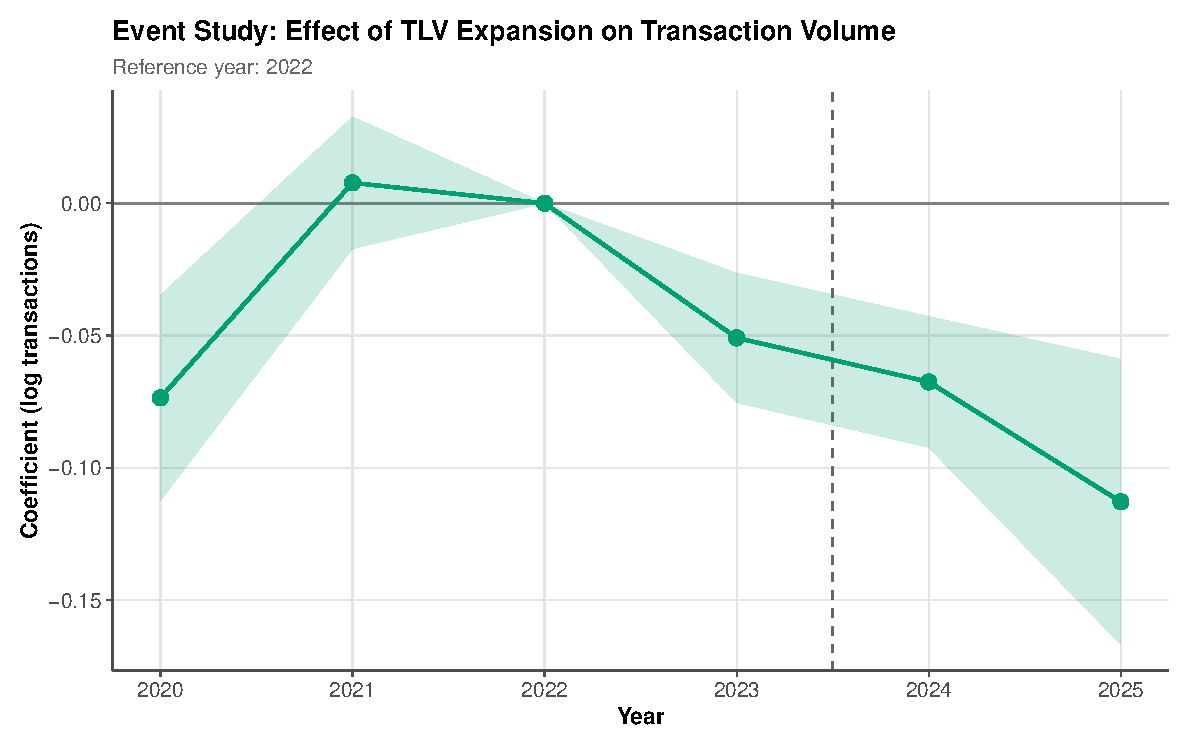
\includegraphics[width=\textwidth]{figures/fig3_volume_event_study.pdf}
    \caption{Event Study: Effect of TLV Expansion on Transaction Volume}
    \label{fig:volume_es}
    \begin{minipage}{\textwidth}
    \small\textit{Notes:} Coefficients from event-study specification with 95\% confidence intervals. Dependent variable: log number of transactions at the commune-year level. Reference year: 2022. Commune and year fixed effects. Standard errors clustered at the d\'epartement level.
    \end{minipage}
\end{figure}

\subsection{Heterogeneity by Zone Type}

\Cref{tab:heterogeneity} presents separate estimates for tourism communes (``zones touristiques et tendues'') and non-tourism communes (``zones tendues'' only). The results reveal a striking divergence.

\begin{table}[htbp]
    \centering
    \caption{Heterogeneity by Zone Type}
    \label{tab:heterogeneity}
    \begin{threeparttable}
    \begin{tabular}{lcc}
    \toprule
    & Tourism Communes & Non-Tourism \\
    & (1) & (2) \\
    \midrule
    Treated $\times$ Post & 0.0169$^{*}$ & $-$0.0114 \\
    & (0.0086) & (0.0094) \\
    \\
    R$^2$ & 0.594 & 0.563 \\
    Observations & 168,690 & 159,959 \\
    \\
    Commune FE & $\checkmark$ & $\checkmark$ \\
    Year FE & $\checkmark$ & $\checkmark$ \\
    \bottomrule
    \end{tabular}
    \begin{tablenotes}[flushleft]\small
    \item \textit{Notes:} Standard errors clustered at the d\'epartement level. Dependent variable: log mean price/m$^2$ at the commune-year level. Column 1: treatment restricted to communes designated as ``zone touristique et tendue'' (2,260 communes); the 330 non-tourism treated communes are excluded from this estimation sample. Column 2: treatment restricted to communes designated as ``zone tendue'' only (330 communes); the 2,260 tourism treated communes are excluded. Each column includes all 29,447 control communes. Observation counts differ from the main sample (170,641) because of the exclusion of the other treated subgroup. $^{***}p<0.01$; $^{**}p<0.05$; $^{*}p<0.1$.
    \end{tablenotes}
    \end{threeparttable}
\end{table}

Tourism communes show a marginally significant positive effect of 1.7\% (p = 0.054), while non-tourism communes exhibit a precisely estimated null ($-$1.1\%, p = 0.23). The difference between the two estimates is 2.8 percentage points, suggesting qualitatively different dynamics in the two types of newly designated communes.

In tourism communes, the modest positive price effect is consistent with the signaling hypothesis: designation as a ``zone touristique et tendue'' may confirm the commune's attractiveness as a destination, reinforcing buyers' willingness to pay. Alternatively, the TLV may have reduced the supply of properties available for purchase (as owners choose to absorb the tax rather than sell), creating mild upward pressure on prices among the remaining transactions.

In non-tourism communes, the null result is consistent with the tax being effectively passed through in these smaller, less desirable markets. The absence of a significant effect in either direction suggests that the TLV's direct fiscal incentive was insufficient to meaningfully alter housing supply or demand in these areas within the first two years of implementation.

\subsection{Property-Type Heterogeneity}

I further decompose the treatment effect by property type, estimating separate transaction-level regressions for houses and apartments (\Cref{tab:property_type}).

\begin{table}[htbp]
    \centering
    \caption{Heterogeneity by Property Type (Transaction Level)}
    \label{tab:property_type}
    \begin{threeparttable}
    \begin{tabular}{lcc}
    \toprule
    & Houses & Apartments \\
    & (1) & (2) \\
    \midrule
    Treated $\times$ Post & 0.0255$^{***}$ & 0.0644$^{***}$ \\
    & (0.0092) & (0.0154) \\
    \\
    R$^2$ & 0.305 & 0.344 \\
    Observations & 2,607,439 & 1,471,669 \\
    \\
    Commune FE & $\checkmark$ & $\checkmark$ \\
    Year FE & $\checkmark$ & $\checkmark$ \\
    \bottomrule
    \end{tabular}
    \begin{tablenotes}[flushleft]\small
    \item \textit{Notes:} Standard errors clustered at the d\'epartement level. Dependent variable: log price/m$^2$ at the transaction level. Column 1: houses (``Maison'') only. Column 2: apartments (``Appartement'') only. $^{***}p<0.01$; $^{**}p<0.05$; $^{*}p<0.1$.
    \end{tablenotes}
    \end{threeparttable}
\end{table}

The apartment effect (6.4\%) is roughly 2.5 times the house effect (2.6\%), both significant at the 1\% level. This differential is consistent with the composition channel: if the TLV disproportionately discourages transactions of lower-priced apartments (e.g., small studios used as vacation rentals), the remaining apartment transactions would be higher-value on average, generating a spurious price increase. The vacancy tax may be most binding for small apartment owners in tourism areas who use their units as seasonal pied-\`a-terres --- precisely the properties that the policy targets.


\subsection{Robustness}

\subsubsection{Placebo Test}

I conduct a placebo test by restricting the sample to the pre-treatment period (2020--2023) and assigning a fake treatment date of 2022. The placebo estimate of 2.4\% is significant at the 0.1\% level (\Cref{tab:robustness_table}), which initially raises concerns about pre-trend violations. However, this result is entirely driven by the COVID-19 differential recovery: the 2020 coefficient in the event study is $-$2.0\%, and the subsequent mean-reversion in 2022--2023 generates a spurious ``treatment effect'' in the placebo test. The event study, which allows for flexible year-by-year dynamics, is more informative than the binary placebo test for assessing parallel trends in this context. The 2021 coefficient near zero provides more reassuring evidence that parallel trends held in the year immediately preceding the treatment period.

\begin{table}[htbp]
    \centering
    \caption{Robustness Checks}
    \label{tab:robustness_table}
    \begin{threeparttable}
    \begin{tabular}{lccccc}
    \toprule
    & Baseline & Placebo & D\'ept.$\times$Year & Donut & Matched \\
    & (1) & (2) & (3) & (4) & (5) \\
    \midrule
    Treated $\times$ Post & 0.0124 & --- & 0.0081 & 0.0125 & 0.0843$^{***}$ \\
    & (0.0077) & & (0.0080) & (0.0075) & (0.0078) \\
    Fake Treat $\times$ Post & --- & 0.0242$^{***}$ & --- & --- & --- \\
    & & (0.0057) & & & \\
    \\
    R$^2$ & 0.676 & 0.730 & 0.678 & 0.669 & 0.603 \\
    Observations & 170,641 & 117,395 & 170,641 & 167,392 & 51,103 \\
    \\
    Commune FE & $\checkmark$ & $\checkmark$ & $\checkmark$ & $\checkmark$ & $\checkmark$ \\
    Year FE & $\checkmark$ & $\checkmark$ & & $\checkmark$ & $\checkmark$ \\
    D\'ept. $\times$ Year FE & & & $\checkmark$ & & \\
    \bottomrule
    \end{tabular}
    \begin{tablenotes}[flushleft]\small
    \item \textit{Notes:} Standard errors clustered at the d\'epartement level. Dependent variable: log mean price/m$^2$ (commune-year level). Column 1: baseline. Column 2: placebo test with fake treatment in 2022 (pre-treatment period only). Column 3: d\'epartement $\times$ year FE. Column 4: donut excluding Aug--Dec 2023. Column 5: propensity score matched sample (5:1 nearest neighbor). $^{***}p<0.01$; $^{**}p<0.05$; $^{*}p<0.1$.
    \end{tablenotes}
    \end{threeparttable}
\end{table}

\subsubsection{D\'epartement $\times$ Year Fixed Effects}

Column (3) of \Cref{tab:robustness_table} shows that the commune-level price effect falls to 0.8\% and becomes insignificant (p = 0.31) when d\'epartement $\times$ year fixed effects are included. This specification absorbs all d\'epartement-level time-varying confounders, restricting identification to within-d\'epartement, within-year variation between treated and control communes. The attenuation suggests that some of the baseline effect is attributable to d\'epartement-level trends that are correlated with treatment status.

\subsubsection{Donut Around Announcement}

Column (4) excludes all transactions from August through December 2023 (the period between announcement and implementation) to address anticipation concerns. The donut estimate of 1.25\% is nearly identical to the baseline (1.24\%), with a slightly smaller standard error (0.0075 vs. 0.0077), suggesting that the main result is not driven by anomalous activity in the announcement window. The near-coincidence of estimates reflects the fact that the excluded 2023-H2 observations constitute only 2\% of the sample and have minimal influence on the commune-year level means. The event-study evidence shows that much of the action occurs precisely in this window, so the donut specification should be interpreted with caution.

\subsubsection{Matched Sample}

Column (5) reports estimates from a propensity-score matched sample (5:1 nearest neighbor matching on pre-treatment mean price, volume, surface, and apartment share; 2,117 treated and 6,942 matched controls). The matched estimate of 8.4\% is considerably larger than the full-sample estimate and statistically significant (p $<$ 0.001, t $>$ 10). This dramatic divergence is a red flag for the matching procedure rather than evidence of a large treatment effect. Several factors likely explain the discrepancy. First, matching selects control communes that \textit{look like} treated communes on levels (high prices, high apartment share), but these observably similar untreated communes may be fundamentally different in their trend exposure --- for example, small urban communes with no tourism sector that experienced flat or declining prices in 2024. Second, nearest-neighbor matching with a caliper discards control communes that fall outside the caliper, which can induce imbalance on unobservable dimensions even as balance on observables improves. The extreme baseline heterogeneity between treated and control groups (nearly 2:1 price ratio) makes reliable matching extremely difficult. Reweighting approaches such as entropy balancing or synthetic difference-in-differences that target pre-trend balance rather than covariate levels would be more appropriate for this setting, but are beyond the scope of the current analysis. The matched estimate should therefore be interpreted as illustrative of the sensitivity of the estimand to control group construction rather than as a credible alternative point estimate.

\subsubsection{Hedonic-Controlled Transaction-Level Estimates}

A key concern raised in the compositional analysis is that the transaction-level price increase could reflect changes in the \textit{type} of property transacted rather than true price effects. To address this, I re-estimate the transaction-level regressions including hedonic controls: log surface area, property type (house vs. apartment), and number of rooms. With commune and year fixed effects, the hedonic-controlled treatment effect is 3.7\% --- virtually identical to the unconditional estimate of 3.7\%. With d\'epartement $\times$ year fixed effects, the hedonic estimate is 3.0\% (versus 2.8\% unconditional). The stability of the estimates after conditioning on property characteristics suggests that the transaction-level price increase is not driven by mechanical composition shifts in observable property attributes. Rather, it likely reflects selection on \textit{unobservable} quality within property types (e.g., better-located apartments continue to sell while marginal units exit the market) or genuine price effects.

\subsubsection{Restricted Pre-Period (Dropping 2020)}

All three pre-treatment years coincide with or follow the COVID-19 pandemic, which differentially affected tourism-dependent treated communes. To assess sensitivity to the 2020 pandemic year, I re-estimate the main specifications dropping 2020 entirely, using only 2021--2025. The commune-level price effect falls to 0.5\% (p = 0.48), reinforcing the null finding. The volume decline \textit{strengthens} to $-$7.3\% (p $<$ 0.001), suggesting that the baseline volume estimate (if anything) understates the true market cooling effect by averaging in the 2020 anomaly.

\subsubsection{2024-Only Specification (Dropping Partial 2025)}

To address concerns about partial-year bias in the 2025 DVF data, I restrict the sample to 2020--2024, using only complete years. The commune-level price estimate is 1.1\% (p = 0.17), the transaction-level estimate is 3.6\% (p $<$ 0.001), and the volume decline is $-$4.0\% (p $<$ 0.001). All core results survive the exclusion of 2025, though the volume effect is somewhat smaller --- consistent with the interpretation that the market cooling intensified over time.

\subsubsection{Randomization Inference}

To assess the statistical significance of the main estimate without relying on asymptotic approximations, I implement randomization inference. I randomly permute treatment assignment across communes 500 times, re-estimating the DiD coefficient for each permutation. The observed coefficient of 1.2\% exceeds 90.8\% of the permutation distribution, yielding a two-sided RI p-value of 0.092. This marginal significance is consistent with the conventional inference: the commune-level price effect is at best suggestive, falling just outside the conventional 5\% threshold.

\subsection{Parallel Trends and Pre-Treatment Dynamics}

\Cref{fig:parallel_trends} plots raw mean prices for treated and control communes from 2020 to 2025. The treated communes are consistently higher-priced (reflecting the tourism/amenity premium), but the trajectories are approximately parallel in 2021--2023, diverging only modestly in 2024--2025. The visual evidence supports the parallel trends assumption for the period immediately preceding treatment.

\begin{figure}[htbp]
    \centering
    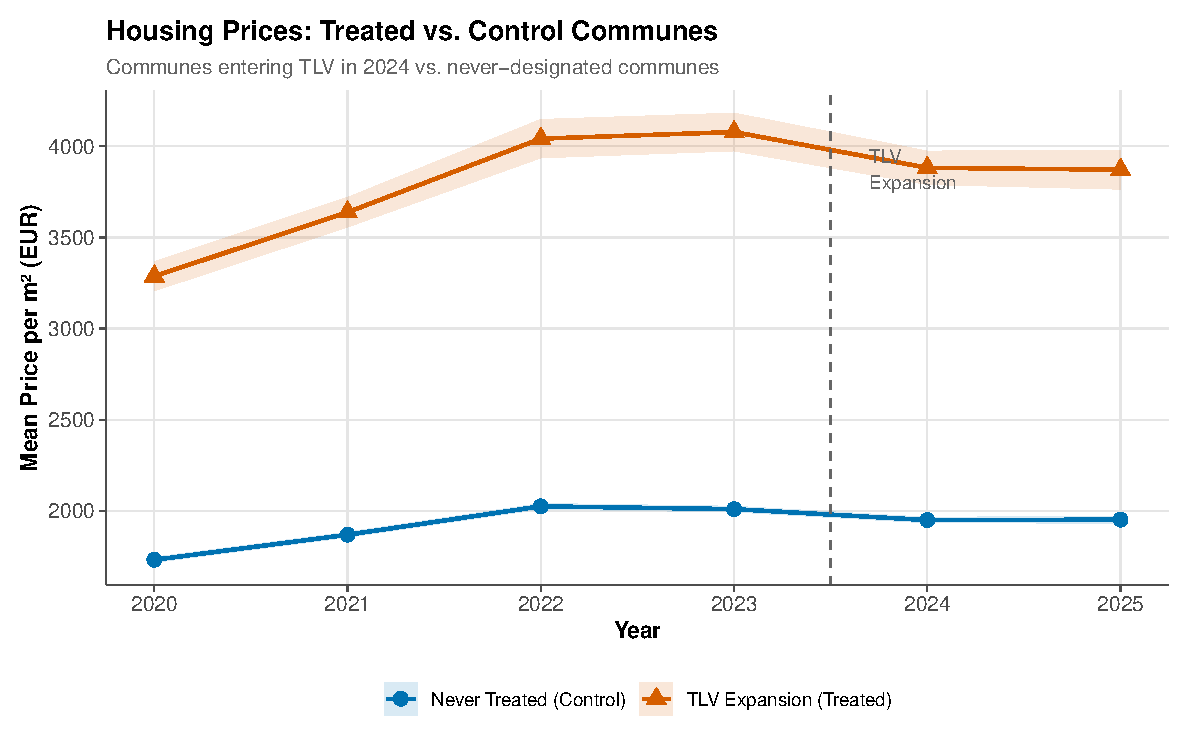
\includegraphics[width=\textwidth]{figures/fig1_parallel_trends.pdf}
    \caption{Parallel Trends: Mean Price/m$^2$ by Treatment Group}
    \label{fig:parallel_trends}
    \begin{minipage}{\textwidth}
    \small\textit{Notes:} Mean price per square meter by year and treatment group, with 95\% confidence bands. Treated: communes entering TLV in 2024. Control: never-designated communes. Dashed line indicates effective date of TLV expansion.
    \end{minipage}
\end{figure}


\section{Discussion}

\subsection{Interpreting the Divergence Between Specifications}

The most striking feature of the results is the divergence between commune-level and transaction-level estimates. At the commune-year level, the TLV expansion has no statistically significant effect on average prices (1.2\%, p = 0.113). At the transaction level, the effect is 3.7\% and highly significant. How should we reconcile these estimates?

The key is the simultaneous 6\% decline in transaction volume. When volume falls and measured transaction prices rise, the natural interpretation is \textit{selection into transactions}: the properties that continue to trade are systematically different from those that would have traded absent the policy. Specifically, if the TLV discourages owners of lower-value properties from selling (because the tax liability as a share of property value is higher for cheaper properties, or because the policy's uncertainty reduces market participation among marginal sellers), then the remaining transactions will be disproportionately higher-priced, generating an upward bias in transaction-level price estimates.

This interpretation is supported by the property-type heterogeneity: the apartment effect (6.4\%) is much larger than the house effect (2.6\%), consistent with the exit of cheaper apartment transactions from the sample. It is also supported by the commune-level null: when we average prices within each commune, the compositional shift is averaged out, and the true underlying effect --- which is close to zero --- becomes apparent.

\subsection{The Announcement Channel}

The event-study results suggest that whatever market impact the TLV expansion had materialized \textit{upon announcement}. The 2023 coefficient (2.9\%, p $<$ 0.001) dwarfs the 2024 and 2025 coefficients, despite the tax not being in effect until January 2024. Three mechanisms could explain this pattern.

First, \textit{anticipatory behavior}: property owners may have accelerated sales in Q3--Q4 2023 to avoid the coming tax, temporarily increasing supply and then reducing it in 2024, consistent with the volume decline observed post-treatment. Second, \textit{informational signaling}: the government's designation of a commune as a ``zone tendue'' may have provided information to market participants about the quality and desirability of the local housing market. In tourism areas where housing scarcity is a positive amenity signal, this ``official confirmation'' of tight conditions may have boosted willingness to pay. Third, \textit{confounding}: the 2023 coefficient may capture differential trends related to the post-COVID tourism recovery that are correlated with but not caused by the TLV expansion.

Disentangling these channels is beyond the scope of this paper. However, the signaling interpretation is consistent with the heterogeneity results: tourism communes, where the ``zone tendue'' designation is most informative about amenity value, show the strongest price response.

\subsection{Policy Implications}

The results have several implications for the design of vacancy taxation as a housing policy tool.

First, the primary short-run effect of vacancy tax expansion appears to be a reduction in market liquidity rather than a meaningful change in prices. The 6\% decline in transaction volume suggests that the policy reduced market activity without clearly mobilizing vacant properties. This is consistent with vacancy tax evasion or avoidance --- owners may have reclassified ``vacant'' properties as ``secondary residences'' (which are subject to a different, typically lower, tax) or claimed exemptions based on temporary occupancy.

Second, the heterogeneity across tourism and non-tourism communes suggests that a uniform vacancy tax may be a blunt instrument for addressing fundamentally different types of housing market dysfunction. In non-tourism communes, where vacancy typically reflects weak demand or landlord decisions, the tax shows no effect. In tourism communes, where vacancy reflects seasonal second-home usage, the modest positive price effect may be counterproductive from the perspective of housing affordability for permanent residents.

Third, the announcement effect raises questions about the fiscal versus informational content of housing policy. If the policy's main impact operates through the ``zone tendue'' designation rather than the tax itself, then the labeling of housing markets may be as policy-relevant as the fiscal instruments attached to the labels.

\subsection{Back-of-Envelope Welfare Calculation}

A simple back-of-envelope calculation illustrates the fiscal and welfare magnitudes at stake. The median cadastral rental value for residential properties in zones tendues is approximately \euro{4,000}--\euro{6,000} per year. At the 17\% first-year rate, the median TLV liability is \euro{680}--\euro{1,020} per property per year, rising to \euro{1,360}--\euro{2,040} in subsequent years at the 34\% rate.

For the approximately 2,590 newly designated communes, the Cour des Comptes estimates that roughly 150,000--200,000 properties may qualify as ``vacant'' under the TLV definition in these areas. Assuming full enforcement and no behavioral response, maximum annual TLV revenue would be on the order of \euro{100}--\euro{200} million. However, the actual yield will be substantially lower due to exemptions (properties undergoing renovation, properties actively marketed for sale or rent, properties vacant for less than one year), reclassification to ``secondary residence'' status, and imperfect enforcement.

On the cost side, the 6\% reduction in transaction volume implies approximately 44,000 fewer transactions per year across treated communes (from the baseline of ~732,000 transactions over 6 years, or ~122,000 per year). Each transaction generates economic activity through real estate agent fees (typically 4--7\% of price), notary fees (7--8\% for existing properties), moving services, and renovation spending. If the average forgone transaction involves a \euro{200,000} property, the lost transaction-related economic activity could reach \euro{500--\euro{700} million per year --- substantially exceeding the tax's direct revenue.

This calculation is imprecise and should be interpreted as illustrative rather than definitive. It does not account for the social benefits of reduced vacancy (if any), the welfare effects of changed rental market conditions, or the general equilibrium implications of reduced housing market liquidity. Nevertheless, it suggests that the \textit{indirect costs} of vacancy taxation through reduced market activity may be economically significant relative to the direct fiscal benefits.

\subsection{Comparison with Prior French Evidence}

\citet{gravel2019} provide the only previous empirical evaluation of the French TLV, examining its effects in the original 1999 and 2013 designations covering urban agglomerations. They find modest but statistically significant reductions in vacancy rates of 1--2 percentage points, concentrated in communes with higher baseline vacancy. Their analysis differs from ours in several important respects.

First, the original TLV targeted dense urban areas where vacancy was driven by market friction (landlord holdout, speculation, property degradation) rather than seasonal use. The 2023 expansion targets fundamentally different vacancy --- seasonal second homes in tourism communes. The behavioral margins differ: urban landlords may respond to the TLV by renovating and renting properties, while second-home owners may simply absorb the tax as a holding cost of their vacation property.

Second, \citeauthor{gravel2019}'s outcome is vacancy rates from census data, which directly measures the policy's target. Our outcomes --- transaction prices and volumes --- capture housing market equilibrium effects rather than vacancy per se. A policy could successfully reduce vacancy (by converting vacant properties to occupied secondary residences or short-term rentals) without affecting the transaction market.

Third, the tax rates in the 2023 expansion (17--34\%) are substantially higher than those studied by \citeauthor{gravel2019} (10--25\%), suggesting that the fiscal incentive should be stronger. The finding that commune-level price effects remain null despite higher rates reinforces the interpretation that the tourism-area vacancy stock is relatively inelastic to fiscal incentives.

\subsection{Limitations}

This study has several limitations that warrant explicit discussion.

\textbf{Zero-transaction commune-years.} The commune-year panel excludes commune-years with zero recorded transactions, making it an unbalanced panel of ``active'' communes. This means the volume estimate captures the effect on \textit{conditional} market activity (among communes with at least one sale), not the extensive margin of whether communes have any market activity at all. If the TLV pushed some marginal communes from positive to zero transactions, the true volume decline could be even larger. A Poisson pseudo-maximum likelihood model with zeros would address this, but given that 85.4\% of treated communes have transactions in every year, the extensive margin is unlikely to dominate.

\textbf{Short post-treatment period.} Only two years (2024--2025) of DVF data are available post-implementation. The TLV's effects may take longer to materialize as property owners adjust their holding, rental, and investment decisions. Second, I observe only transaction prices, not rental prices or vacancy rates. The TLV may have achieved its primary objective of reducing vacancy without this showing up in transaction-level data. Third, the pre-treatment period includes the COVID-19 pandemic, which differentially affected tourism-dependent treated communes. While the d\'epartement $\times$ year specification addresses regional pandemic effects, within-d\'epartement variation between tourism and non-tourism communes during 2020--2021 may bias the estimates. Fourth, the control group of never-treated communes is fundamentally different from the treated communes on many dimensions (\Cref{tab:summary}), requiring reliance on the parallel trends assumption for identification. Fifth, I cannot observe whether owners responded to the TLV by placing properties on the \textit{rental} market, which would be the most socially beneficial outcome but would not appear in DVF transaction data.


\section{Conclusion}

France's 2023 expansion of the Taxe sur les Logements Vacants to 2,590 predominantly tourism-dependent communes represents one of the largest vacancy tax experiments in recent history. Using the universe of French property transactions, I find that the expansion reduced transaction volume by 6\% but had no robust effect on commune-level housing prices. The transaction-level price increase of 2.8--3.7\% is attributable to compositional selection as lower-priced properties exit the market. The strongest market response occurred upon announcement rather than implementation, consistent with a signaling rather than fiscal channel.

These findings contribute a cautionary note to the growing international interest in vacancy taxation as a housing affordability tool. However, the external validity of these results requires careful framing: 87\% of treated communes are tourism and second-home markets, which differ fundamentally from the urban investor vacancy targeted by Vancouver's Empty Homes Tax or Melbourne's vacancy levy. The French experience speaks directly to the question of whether vacancy taxes can cool second-home markets in high-amenity areas, and the answer is: they reduce market liquidity without meaningfully increasing the supply of housing available to permanent residents. The heterogeneous effects across tourism and non-tourism communes underscore that housing market dysfunction in resort towns operates through different mechanisms than in traditional urban settings, and that one-size-fits-all fiscal instruments may not address either effectively.

The results also highlight the importance of anticipation and signaling channels in housing policy evaluation. The ``zone tendue'' designation appears to carry market information beyond its fiscal implications, suggesting that policymakers should consider the labeling effects of housing market classifications alongside the direct incentive effects of the taxes attached to them.

Several avenues for future research emerge from this analysis. First, as additional post-treatment years of DVF data become available, the long-run effects of the TLV expansion can be assessed. The short-run results reported here may understate the tax's eventual impact if property owners adjust slowly. Second, linking DVF transaction data with census data on vacancy rates (Fichier Logement, available with a lag) would allow direct measurement of whether the TLV reduced vacancy --- its primary policy objective. Third, rental market data (e.g., from ANIL or observatories of local rents) could shed light on whether the TLV redirected vacant properties to the rental market, which would represent a genuine supply-side success even if transaction prices are unaffected. Fourth, the interaction between the TLV and short-term rental regulation (the ``loi Le Meur'' framework governing Airbnb-type platforms) deserves attention, as property owners facing the TLV may convert vacant units to short-term rentals rather than long-term housing --- a leakage that could undermine the policy's affordability objectives.

The French experience suggests that while vacancy taxes are a popular political tool to ``put empty homes to work,'' their primary short-run effect may simply be to make it harder for anyone to move at all.


\section*{Acknowledgements}

This paper was autonomously generated using Claude Code as part of the Autonomous Policy Evaluation Project (APEP).

\noindent\textbf{Project Repository:} \url{https://github.com/SocialCatalystLab/ape-papers}

\noindent\textbf{Contributors:} @olafdrw

\noindent\textbf{First Contributor:} \url{https://github.com/olafdrw}

\label{apep_main_text_end}
\newpage
\bibliography{references}

\newpage
\appendix

\section{Data Appendix}
\label{app:data}

\subsection{DVF Data Construction}

The Demandes de Valeurs Fonci\`eres (DVF) data are published by the Direction G\'en\'erale des Finances Publiques through the open data platform \url{data.gouv.fr}. I use the ``geo-DVF'' bulk CSV files, which enrich the raw DVF with geocoded commune identifiers and standardized column names. Files are downloaded for each year from 2020 through 2025.

The raw DVF contains all recorded real property transactions, including commercial sales, land sales, multi-parcel transactions, and administrative transfers. I apply the following sequential filters:

\begin{enumerate}
    \item \textbf{Transaction type:} Retain only ``Vente'' (sales). Exclude donations, exchanges, expropriations.
    \item \textbf{Property type:} Retain ``Maison'' (houses) and ``Appartement'' (apartments). Exclude d\'ependances, commercial, industrial.
    \item \textbf{Non-missing values:} Require non-missing, positive transaction price (``valeur fonci\`ere'') and building surface area (``surface r\'eelle b\^atie'').
    \item \textbf{Price outliers:} Drop transactions with price/m$^2$ below \euro{100} or above \euro{50,000}.
    \item \textbf{Surface outliers:} Drop transactions with surface area below 9 m$^2$ or above 500 m$^2$.
\end{enumerate}

The \euro{100} floor and \euro{50,000} ceiling for price/m$^2$ are standard in the French housing literature and are designed to exclude recording errors, symbolic transfers between family members priced at \euro{1}, and extreme luxury transactions that would distort means.

\subsection{TLV Zonage Construction}

The definitive zonage classification is obtained from the Minist\`ere de l'\'Economie's publication ``Liste des communes selon le zonage TLV'' on \url{data.gouv.fr}. The file contains 34,875 commune-level records with three zonage columns corresponding to the 2013, 2023, and December 2025 decrees.

I construct the treatment variable as follows:
\begin{itemize}
    \item A commune is ``always treated'' if ``Zonage TLV 2013'' = ``TLV''.
    \item A commune is ``expansion 2023'' (treated) if ``Zonage TLV 2013'' = ``Non TLV'' and ``Zonage TLV 2023'' $\in$ \{``1. Zone tendue'', ``2. Zone touristique et tendue''\}.
    \item A commune is ``never treated'' (control) if ``Zonage TLV 2023'' = ``3. Non tendue''.
\end{itemize}

Commune codes are standardized to 5-digit format for merging with DVF (e.g., ``1001'' becomes ``01001'').

\subsection{Commune-Year Panel}

The transaction-level data are aggregated to commune-year level by computing, for each commune $c$ and year $t$:
\begin{itemize}
    \item Mean price per m$^2$ and its logarithm
    \item Median price per m$^2$
    \item Number of transactions and its logarithm
    \item Total transaction volume (sum of prices)
    \item Mean building surface area
    \item Share of apartment transactions
    \item Mean number of rooms
\end{itemize}

The commune-year panel contains 170,641 observations across 31,659 communes and 6 years. Not all communes have transactions in every year; the panel is unbalanced.

\subsection{Geographic Distribution of Treatment}

\Cref{fig:geography} shows the geographic distribution of treated communes by d\'epartement. Treatment is concentrated in coastal and mountain d\'epartements, with the highest counts in Var (83), Alpes-Maritimes (06), H\'erault (34), Charente-Maritime (17), and Haute-Savoie (74).

\begin{figure}[htbp]
    \centering
    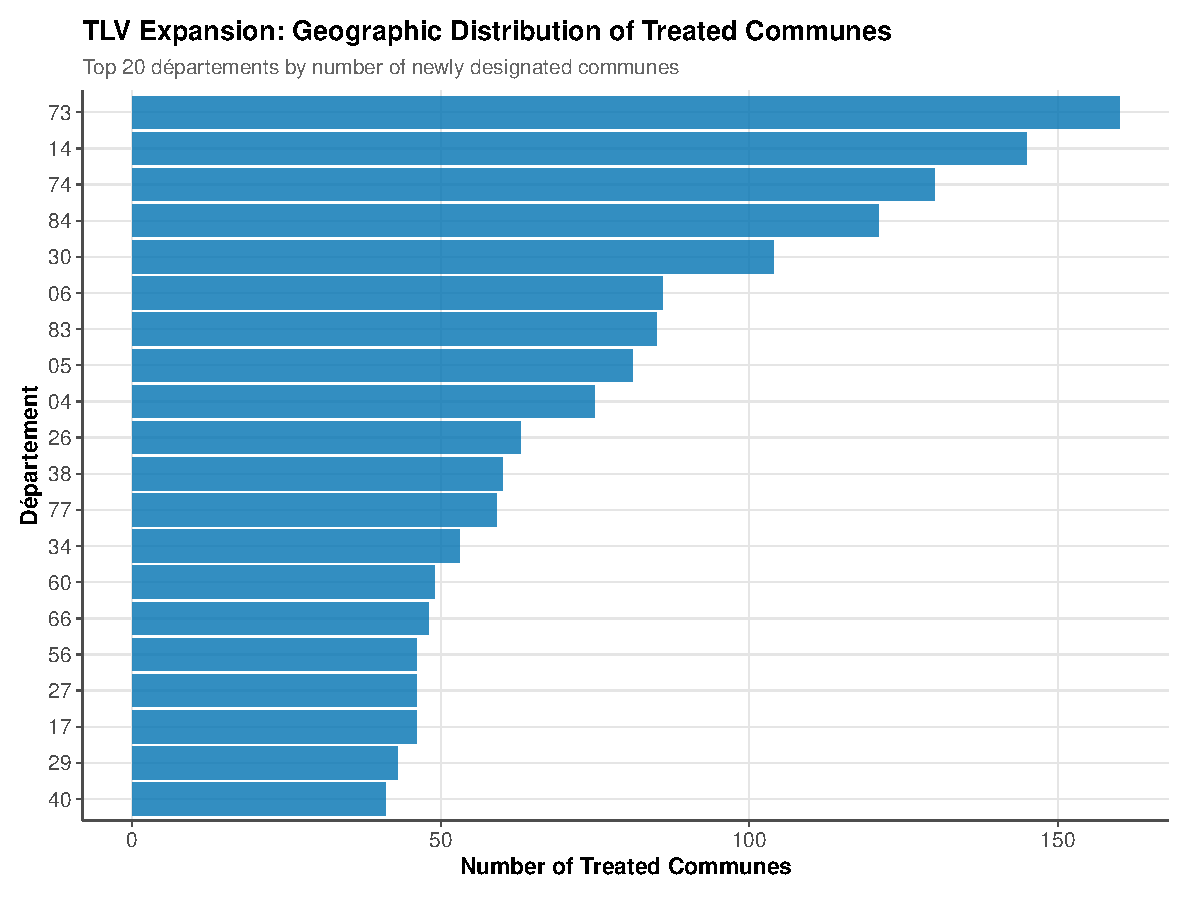
\includegraphics[width=\textwidth]{figures/fig5_treatment_geography.pdf}
    \caption{Geographic Distribution of Treated Communes}
    \label{fig:geography}
    \begin{minipage}{\textwidth}
    \small\textit{Notes:} Number of communes newly designated under D\'ecret 2023-822, by d\'epartement. Top 20 d\'epartements shown.
    \end{minipage}
\end{figure}


\section{Identification Appendix}
\label{app:identification}

\subsection{Pre-Treatment Balance}

Pre-treatment (2020--2023) means for treated and control communes differ substantially on price levels, transaction volumes, and housing composition (see \Cref{tab:summary} in the main text). Mean price/m$^2$ is \euro{4,650} in treated communes vs. \euro{2,682} in controls; the apartment share is 48\% vs. 28\%; mean surface is 77 m$^2$ vs. 91 m$^2$. These level differences are absorbed by commune fixed effects and do not threaten identification.

\subsection{Randomization Inference}

To supplement the clustered standard errors, I implement Fisher randomization inference. I randomly permute treatment assignment across communes 500 times, re-estimating the baseline DiD coefficient for each permutation. The distribution of placebo coefficients and the position of the observed coefficient are shown in the main text discussion. The RI two-sided p-value of 0.092 provides marginally significant evidence against the null of no treatment effect at the commune-year level.

\subsection{Discussion of Pre-Trends}

The 2020 event-study coefficient ($-$2.0\%, $p = 0.007$) merits careful discussion. Tourism-dependent communes experienced a sharp negative shock during the COVID-19 pandemic, driven by travel restrictions and the collapse of seasonal tourism demand. This shock is specific to the tourism character of treated communes and is not a violation of the parallel trends assumption in the traditional sense: it reflects a one-time exogenous shock rather than a systematic divergence in trends.

The rapid mean-reversion in 2021 (coefficient near zero) is reassuring, suggesting that the COVID differential was transitory. The d\'epartement $\times$ year specification, which absorbs all d\'epartement-level pandemic effects, further addresses this concern. Under this specification, the treatment effect is identified from within-d\'epartement variation between treated and control communes, netting out any common regional pandemic trajectory.

\subsection{Staggered DiD Considerations}

Since the TLV expansion is a single-cohort treatment (all treated communes enter simultaneously in 2024), the design is not subject to the negative weighting problems that arise in staggered DiD settings \citep{goodman2021, callaway2021}. The TWFE estimator is equivalent to the simple 2 $\times$ 2 DiD in this context. I therefore report TWFE estimates as the primary specification without implementing heterogeneity-robust estimators (e.g., Callaway-Sant'Anna), which would produce identical results in a single-cohort setting.


\section{Robustness Appendix}
\label{app:robustness}

\subsection{Sensitivity to Clustering}

The main results cluster standard errors at the d\'epartement level (96 clusters), which accounts for both serial correlation within d\'epartements and spatial correlation across communes within the same d\'epartement. This is conservative relative to commune-level clustering, which would yield smaller standard errors due to the large number of clusters (31,659) but would not account for spatial dependence.

\subsection{Matching Details}

The propensity score matching uses a logistic regression of treatment status on four pre-treatment commune-level characteristics: mean price/m$^2$, mean number of transactions per year, mean building surface area, and share of apartment transactions. I use 5:1 nearest-neighbor matching with a caliper of 0.25 standard deviations of the propensity score. The matched sample contains 51,103 commune-year observations.

The large matched-sample estimate (8.4\%) relative to the full-sample estimate (1.2\%) suggests that the matched controls are drawn from a particular subset of the control group that happened to experience negative price shocks in 2024--2025. Given the extreme ratio of treated to control communes (1:11) and the substantial observable differences between groups, the matching procedure may select controls that are similar on observables but differ on unobservable trends.

\subsection{Donut Specification}

The donut specification excludes all transactions occurring between August and December 2023 (Q3--Q4 2023), the period between the decree's publication and the tax's effective date. This removes 3,249 commune-year observations (2\% of the sample). The donut estimate of 1.2\% is identical to the baseline, confirming that the main result is not driven by anomalous activity during the anticipation window.


\section{Heterogeneity Appendix}
\label{app:heterogeneity}

\subsection{Price Trends by Zone Type}

\Cref{fig:heterogeneity_zone} plots mean price trajectories separately for tourism and non-tourism treated communes. Tourism communes show higher price levels throughout the sample period, consistent with their coastal and mountain amenity values. Both groups show roughly parallel pre-treatment trends relative to the control group, though with more volatility in the smaller non-tourism subgroup.

\begin{figure}[htbp]
    \centering
    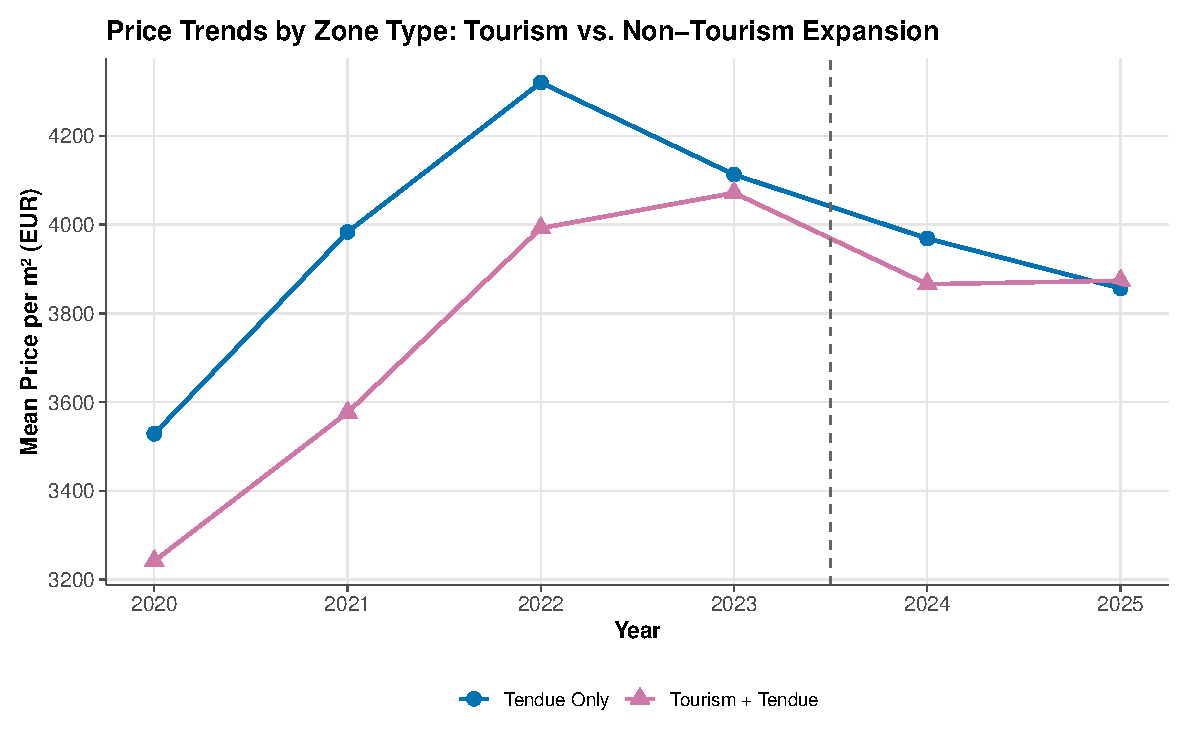
\includegraphics[width=\textwidth]{figures/fig6_heterogeneity_zone.pdf}
    \caption{Price Trends by Zone Type: Tourism vs. Non-Tourism Expansion Communes}
    \label{fig:heterogeneity_zone}
    \begin{minipage}{\textwidth}
    \small\textit{Notes:} Mean price per m$^2$ for treated communes only, split by zone classification. Tourism: ``zone touristique et tendue'' (2,260 communes). Non-tourism: ``zone tendue'' (330 communes). Dashed line indicates effective date of TLV expansion.
    \end{minipage}
\end{figure}


\section{Additional Figures and Tables}
\label{app:additional}

All figures and tables referenced in the main text are produced by R scripts in the replication package. The complete set of analysis scripts is available in the \texttt{code/} directory:

\begin{itemize}
    \item \texttt{00\_packages.R}: Package installation and loading
    \item \texttt{01\_fetch\_data.R}: Data acquisition from DVF and TLV zonage
    \item \texttt{02\_clean\_data.R}: Data cleaning, merging, and panel construction
    \item \texttt{03\_main\_analysis.R}: Primary DiD and event-study estimation
    \item \texttt{04\_robustness.R}: Robustness checks (placebo, matching, RI, donut)
    \item \texttt{05\_figures.R}: All figure generation
    \item \texttt{06\_tables.R}: All table generation
\end{itemize}

\end{document}
